\documentclass[12pt]{article}
\usepackage{graphicx,psfrag,amsmath,amsfonts,verbatim}
\usepackage[small,bf]{caption}
\usepackage{hyperref}

\bibliographystyle{alpha}

\title{Discovering signals in fMRI data; 
a Bayesian nonparametric approach   \\ \large{Progress Report for STAT 30850}}
\author{Ahmed Bou-Rabee, Wanrong Zhu, Zheng Xu, Mo Zhou}

\begin{document}
\maketitle

{\bf Summary of Progress } 

The goal of this project is to formulate and test a method which can be used to adaptively identify  clusters of signals in functional magnetic resonance imaging (fMRI) data. Recall that the fMRI data is in the form (voxel, time, intensity of reading). Inspired by Stephens (2000), we describe a bayesian nonparametric method by creating a Markov birth-death process with stationary distribution to detect clusters of signals. Theoretically, this method works for multiple-dimensional data which incorporates spatial and temporal information.

For now, the performance of the proposed approach is measured through a simulation study. To make it computationally feasible,  our simulated dataset includes two-dimensional spatial data (whereas fMRI data has three dimensions in space and one dimension in time), and corresponding p-values for each entry. The empirical result is promising on the simulated dataset. The clusters of signals are constantly detected from observing the plots. Since it is difficult to test the performance of a method which doesn't have a predefined solution, we will compare the proposed approach against the p-filter, introduced in Barber and Ramdas (2015), to perform the same task on this simulated dataset and it is able to detect the clusters from observing the plots.  Here it arises the first challenge. We need to come up with a quantitative method to measure the accuracy and evaluate the performance. 

Our next step will be to apply the proposed approach on the fMRI data. Other than coming up with a quantitative way to evaluate the algorithm, we also see challenges rising from computational costs given the nature of our approach when dimension increases. A potential idea is to exclude temporal information and only considers spatial information.

\vspace{1em}
{\bf Bayesian Nonparametric Approach}

 Our strategy is to view each cluster as a point in parameter space, and create birth-death process with the posterior distribution of the parameters as its stationary distribution. 
 
 The predefined birth rate $\lambda$ is independent of the clusters, whereas the death rate $\mu_i$ at each step depends on the current clusters. There is a predefined length of time $t$, and within this time frame, "current" clusters are expected to update every step, with probability of "borning" a new cluster of $\frac{\lambda}{\lambda+\mu_i}$ and probability of "killing" an existing cluster of $\frac{\mu_i}{\lambda+\mu_i}$. It worth emphasizing that $u_i$ is updated after each step using the updated clusters. This process ends until predefined time $t$ expires, and it gives us a set of predicted clusters. We repeat this procedure many times, say $10000$, and keep the last $100$ versions of clusters, over which we determine if it is a signal or not.
 
Here we will briefly describe the idea of calculating death rate using "current" clusters. We first compute the log likelihood $l$ of this "current" cluster model. Then we compute the log likelihood $l_{-k}$ of the new cluster model obtained from "killing" cluster $k$. Repeat this for each cluster in the "current" model. It follows that $u_i = \sum_{k=1}{K} e^{\triangle_k}$ where $\triangle_k = l_{-k} - l + constant$ 

We also think about incorporating metropolis-hastings algorithm to sample mixture proportions and beta in each repetition to improve the algorithm.


\vspace{1em}
{\bf Early Empirical Result } 

1. Data and Preliminaries: 

we sample a 100-by-100 grid with 5 clusters of signals and the rest is null. Each entry is denoted as
$d_i = (x_i, y_i, p_i)$ where $x_i$ and $y_i$ are coordinates and $p_i$ is the p-value associated with point $i$. The first step is to generate 5 clusters spatially on the grid. The centers $C_k$ of these 5 clusters are sampled uniformly from the entire grid while being distinct, and the radius $R_k$ are sampled from the Truncated Normal $TN(7, 2, 5,10)$, for k = 1, 2 ..., 5. Next step is to simulate signals in each of the five clusters. We sample $b_k \sim U(2,5)$ and for each $d_i$ in $C_k$, $p_i \sim Beta(\frac{1}{b_k},b_k)$.

Figure 1. shows the simulated data graphically. From the heatmap, we can obviously see there are five clusters with strong signals while the rest is noise. This is confirmed in the histogram of p-values. 

\begin{figure}[h]
\caption{Left is a heatmap of actual data and right is histogram of actual data}
\centering
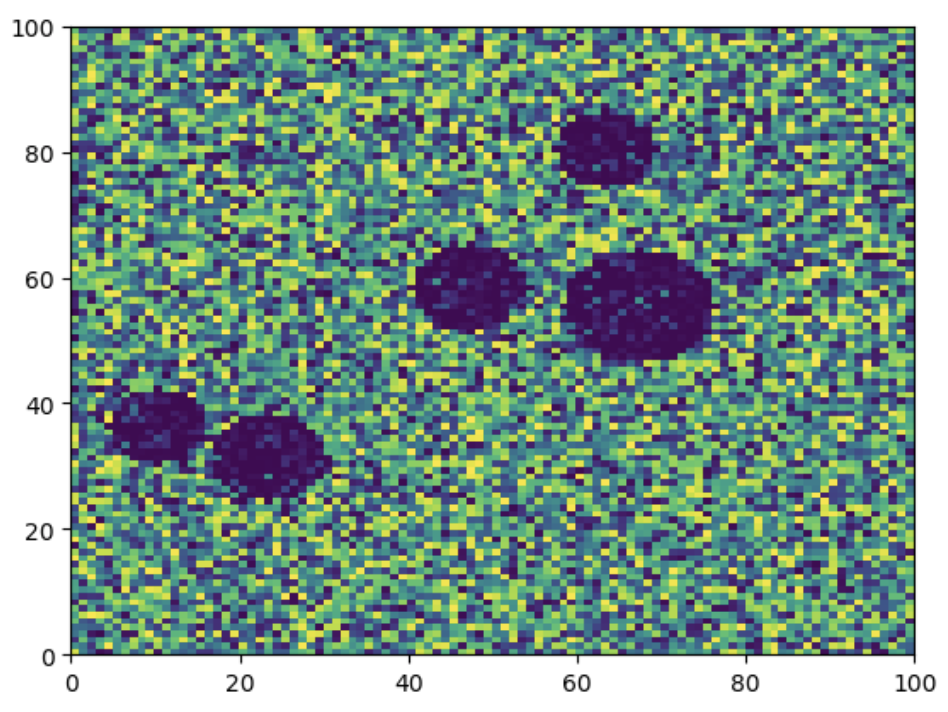
\includegraphics[width=6.5cm]{actualgrid}
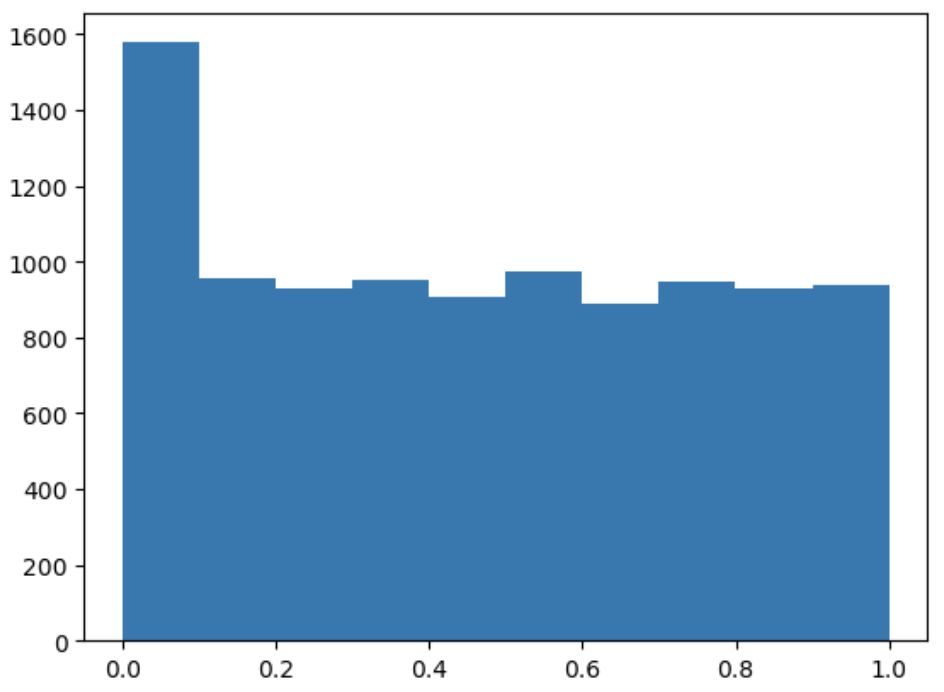
\includegraphics[width=6.5cm]{actualhist}
\end{figure}

\vspace{1em}
2. Priors for Bayesian Analysis: 

We specify priors for the number of clusters $K$, radius of clusters $r$, and beta parameter for Beta distribution as follows: \\
$$K \sim TRUNCATE ( Poisson(50), 1, 100 )$$
$$r \sim TRUNCATE ( Normal(5, 2), 1, 100 )$$
$$\beta \sim TRUNCATE ( Normal(8, 5), 2, 200 )$$
Here we haven't given too much thoughts on good priors. This is will be taken consideration in our next step.

\vspace{1em}
3. Comparison Between Actual and Detected Signals : 

We present the predicted signals using bayesian nonparametric approach (Figure 2.) as well as p-filter algorithm (Figure 3.) on the 100-by-100 grid. Recall that the plots for the actual data is in part 1.
\begin{figure}[h]
\caption{Predictions using bayesian nonparametric approach with location information. Left is heatmap of p-values and right is histgram}
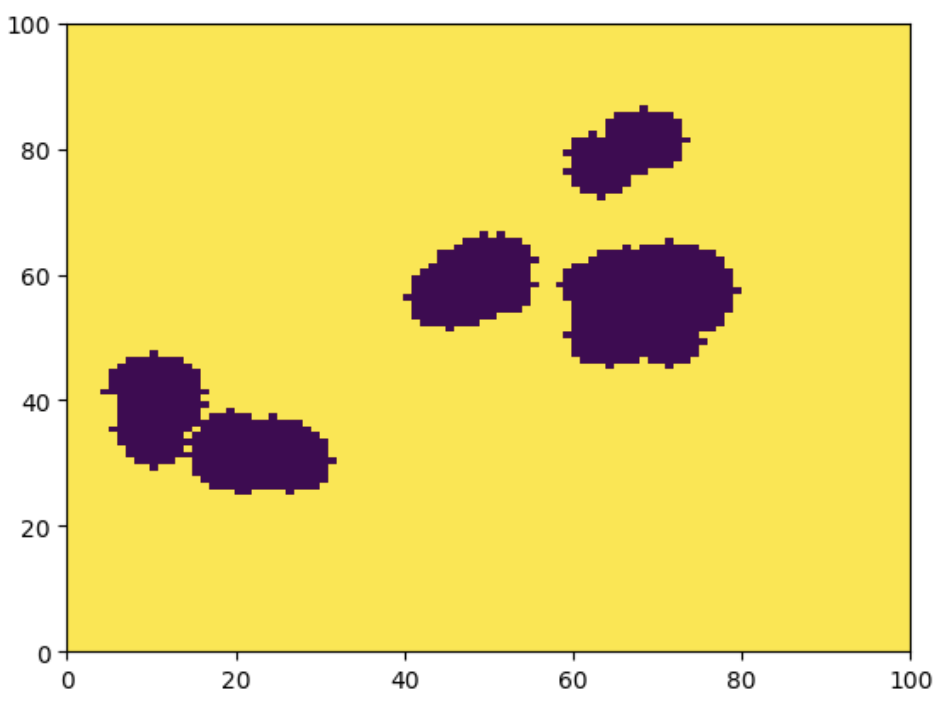
\includegraphics[width=6.5cm]{baygrid}
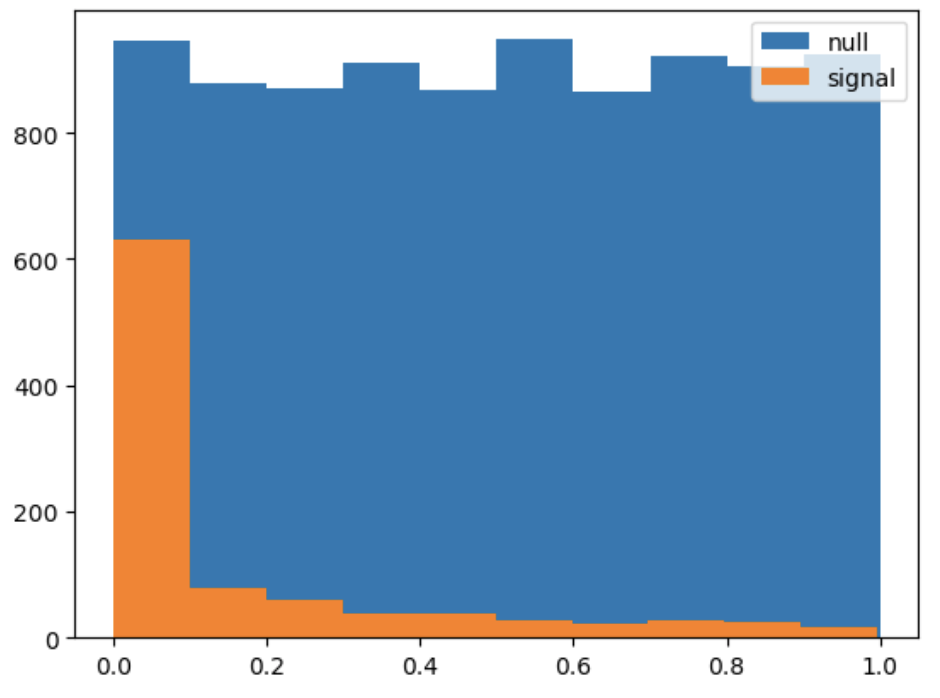
\includegraphics[width=6.5cm]{bayhist}
\end{figure}

\begin{figure}[h]
\caption{Predictions using p-filter}
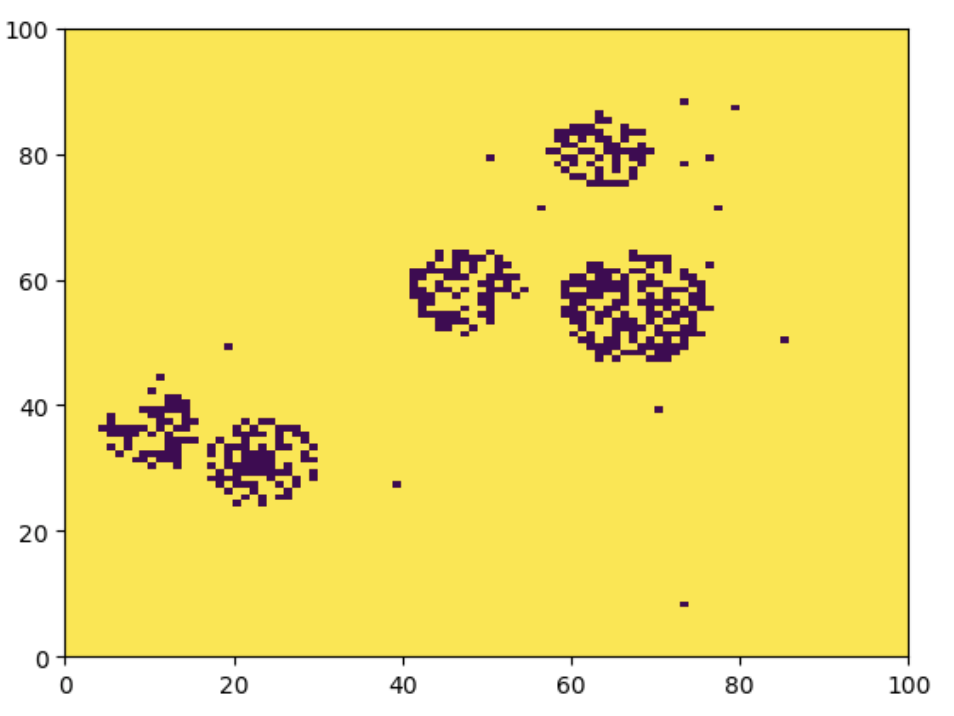
\includegraphics[width=6.5cm]{pfiltergrid}
\end{figure}


\vspace{1em}
{\bf Summary of Future Work and Questions}

1. Propose a reasonable quantitative measurement to compare the clustering results obtained from the proposed approach and the p-filter algorithm 

2. Applying the proposed approach to real fMRI data can be very computationally expensive. Run on server or reduce the problem?

3. Giving better priors to the proposed bayesian approach?

4. Incorporating Metropolis-Hastings algorithm to improve the proposed approach?


\bibliography{bibliography}



\end{document}